% !TEX root = ../../semexp-thesis.tex

\section{The Augmented Exploratory Programming Workflow}
\label{sec:approach/workflow}

\begin{figure}
	\centering
	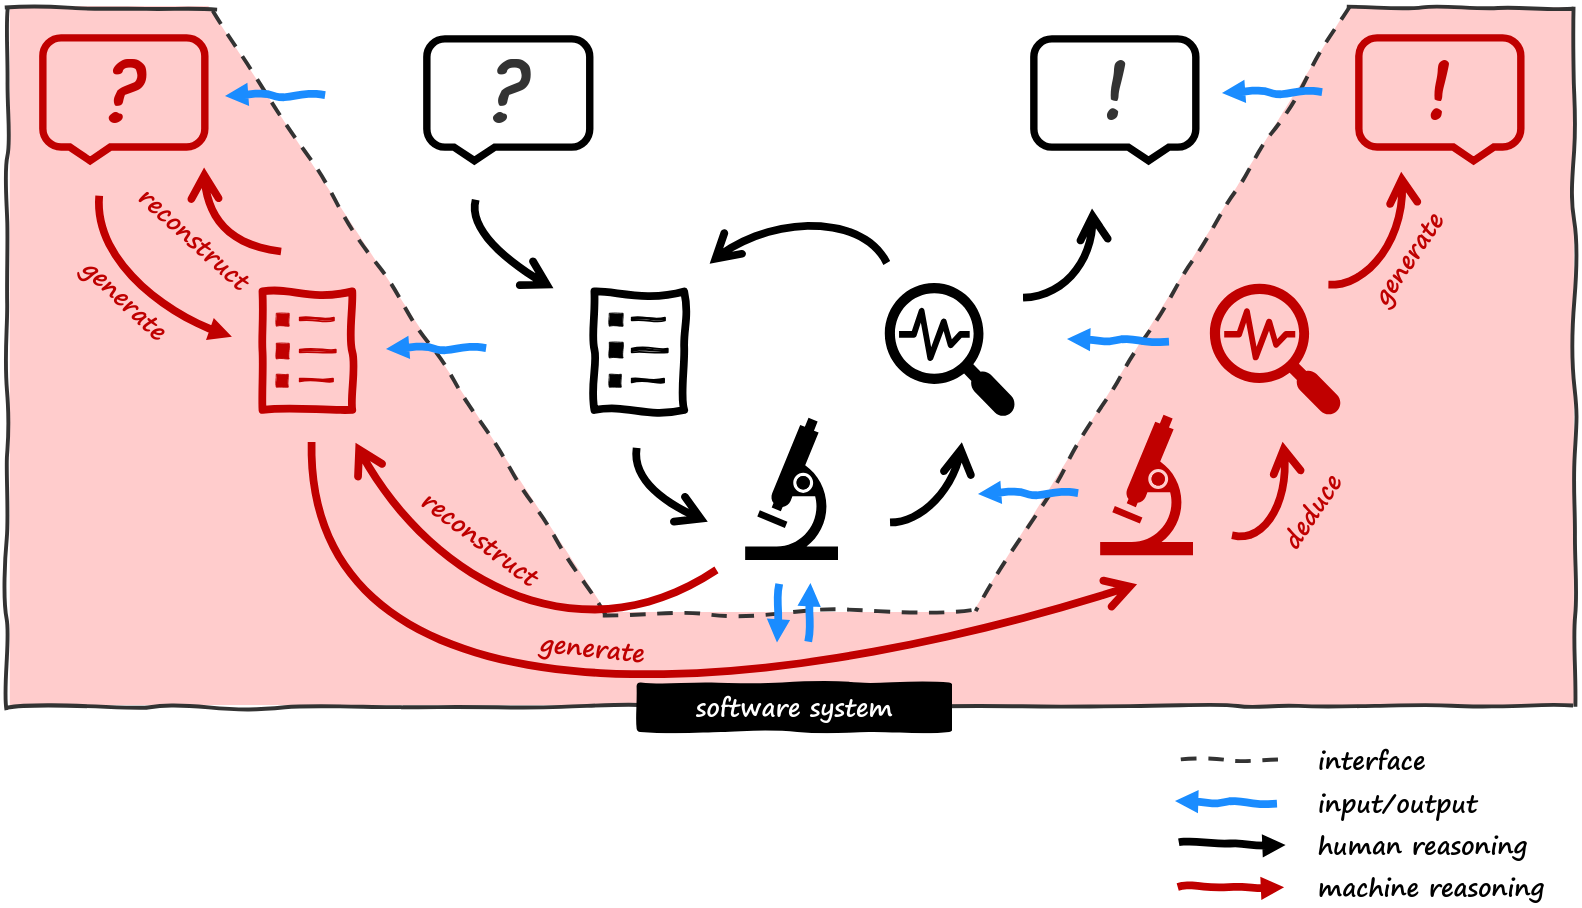
\includegraphics[width=\textwidth]{01_workflow/workflow.png}
	\caption[Our model of an \emph{augmented exploratory programming workflow}.]{
		Our model of an augmented exploratory programming workflow.
		Programmers can exchange conceptual artifacts with a \emph{semantic exploratory programming system} (\bold{\textcolor[HTML]{c00000}{red}}) through high-level semantic interfaces.
		Based on the shared artifacts, the programming system continues the research process and suggests new artifacts to the programmer.
	}
	\label{fig:approach/workflow/workflow}
\end{figure}

In the traditional exploratory programming workflow, programmers receive limited support from programming systems, which causes semantic distances, information overload, and frequent interruptions.
To address these challenges, we propose a new \emph{augmented exploratory programming workflow}, which describes collaborations between programmers and systems at higher abstraction levels and introduces the notion of \emph{semantic exploratory programming systems}, which integrate semantic technologies to support programmers in conceptual research steps such as planning or understanding~(\cref{fig:approach/workflow/workflow}).

In our augmented workflow, programmers can provide semantic context from their research process to the exploratory programming system, such as questions, plans, and previous experiments.
The system builds on this context to ``think along'' and continue the research process on its own:
it attempts to conduct next likely steps such as planning and executing experiments, deducing results, or answering questions and shares its work with the programmer at different granularities.
For example, a programmer could provide a high-level question to the system and receive a list of suggested experiments to execute; or they could perform their own experiments and receive an automated summary of deduced results from the system.
Thus, programmers can either \emph{delegate} tasks to the system to avoid interruptions, or they can \emph{cooperate} with it to benefit from semantic technologies and \emph{augment} their workflow with additional context.

To support this workflow, we propose \emph{semantic exploratory programming systems}:
these systems build upon traditional exploratory programming systems and connect them with semantic technologies to gain access to the semantic context at higher abstraction levels of the research process.
For example, this connection allows exploratory programming systems to interpret questions and plans, contextualize and analyze experiments, or summarize results and answer questions.
Using that context, semantic exploratory programming systems can replicate the previous research steps of programmers and suggest possible next steps.

To access and contribute to the exploratory research process of programmers, semantic exploratory programming systems require new \emph{semantic interfaces}, through which programmers can provide contextual artifacts as inputs and retrieve semantic suggestions and answers as outputs.
Concretely, we propose three types of semantic interface mechanisms:

\begin{description}
	\item[Anticipated experiments:]
	The semantic exploratory programming system observes the \emph{experiments} that the programmer executes through traditional interfaces.
	Based on these observations, it attempts to reconstruct their underlying plans and uses these plans to anticipate and suggest further experiments to the programmer.

	\item[Semantic inputs:]
	The semantic exploratory programming system reinterprets existing or introduces new interfaces, through which programmers can express their current \emph{plans}.
	For example, this involves reading quick notes of programmers (such as to-do lists kept in a workspace), observing the setup of experiments before the programmer executes them, or---hypothetically---even listening to programmers thinking out loud during their work.
	Based on these inputs, the system can develop a more precise understanding of the programmer's plans and provide more relevant suggestions to them.

	Furthermore, the system can also attempt to reconstruct the overarching \emph{question} of the programmer based on the provided plans.
	This serves as a base for anticipating further plans and developing suggestions for them even before programmers express these plans to the system.

	Finally, the system can offer new interfaces, through which programmers can explicitly express high-level questions.
	The system can use these to refine existing and new plans and provide more contextualized suggestions.

	\item[Semantic outputs:]
	Based on conceptualized ideas and questions, the semantic exploratory programming system can provide suggestions to programmers through new output interfaces at different abstraction levels.
	It can suggest low-level \emph{experiments} or execute them on its own and automatically deduce and summarize \emph{results}.
	If the system knows the original question of the programmer, it can also consolidate and contextualize results to provide a direct \emph{answer} to this question.
\end{description}

Internally, semantic technologies are used to reconstruct plans and questions of programmers, make suggestions, and deduce results and answers.
\Cref{cha:suggestions} describes how text embeddings and semantic retrieval are employed to anticipate plans and experiments, and \cref{cha:agent} explains how systems can use generative LLMs to interpret questions, generate experiments, and deduce answers.
